\documentclass{article}

\usepackage[utf8]{inputenc}
\usepackage[T1]{fontenc}
\usepackage{microtype}

\usepackage{newspaper}
%% [LianTze] Contains some modifications
\usepackage{paper-mod}
%%... so now you can redefine the headline and byline style if you want to.
%% These can be issued just before any
%% byline or headline in the paper, to
%% individually style each article
%%
% \renewcommand{\headlinestyle}{\itshape\Large\lsstyle}
% \renewcommand{\bylinestyle}{\bfseries\Large\raggedright}


\date{\today}
\currentvolume{1}
\currentissue{2}

%% [LianTze] The newspaper package also provides 
%% these commands to set various metadata:

%% The banner headline on the first page
%%   (The colon after s: is to get a more
%%   modern majuscule s in this font instead of 
%%   the medieval tall s. For anyone interested 
%%   in the history: 
%%  http://medievalwriting.50megs.com/scripts/letters/historys.htm)
\SetPaperName{Liberty City Outsider}

%% The name used in the running header after
%% the first page
\SetHeaderName{Transformation news}

%% and also...
\SetPaperLocation{The Guild}
\SetPaperSlogan{Первый пролетарский вестник}
\SetPaperPrice{Free}


% [LianTze] times (the package not the font) is rather outdated now; use newtx (see later)
% \usepackage{times}
\usepackage{graphicx}
\usepackage{wrapfig}
\usepackage{multicol}

\usepackage{picinpar}
%uasage of picinpar:
%\begin{window}[1,l,\includegraphics{},caption]xxxxx\end{window}


%%%%%%%%%  Front matter   %%%%%%%%%%

\usepackage{lipsum}

\begin{document}

\maketitle

\begin{multicols}{3}

\headline{\bf\sf\Large Коллективизация!}
Дружным строем завершаем победу в деле социалистической переделки процессов разработки. Все в фичатимы, товарищи!
\\\\Подробности на странице 2 >>
\vspace{14mm}
\closearticle

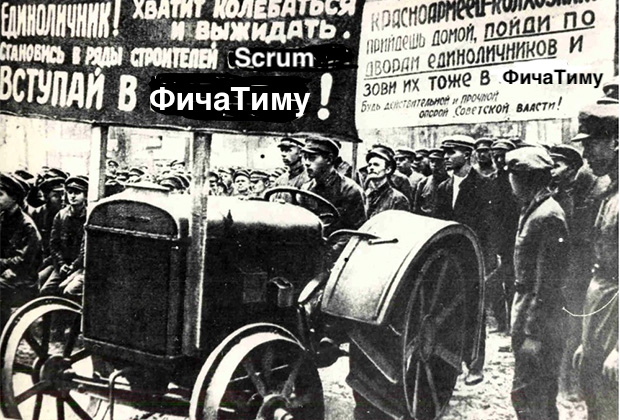
\includegraphics[width=11.2cm]{klh2.jpeg}

\end{multicols}

\begin{multicols}{3}

\headline{\bf\sf\Large Каждый принадлежит всем остальным}
Сервисы теперь общие! Как фантастика Хаксли становится реальностью, а взаимопользование сервисами для доставки своей фичи обыденностью.
\\\\Подробности на странице 2 >>
\closearticle

\headline{\bf\sf\Large Вот тут влетает, а вон там вылетает}
Объясняем в доступной форме не инженерам механизм доставки изменений на бой.
\\\\Подробности на странице 3 >>
\vspace{5mm}
\closearticle

\headline{\bf\sf\Large Вот сюда кидаешь, а вон там ловят}
Объясняем в доступной форме инженерам механизм доставки изменений на бой.
\\\\Подробности на странице 3 >>
\closearticle

\end{multicols}

\begin{multicols}{3}

\headline{\bf\sf\Large Призрак трансформации ходит по репозиториям}
Товарищ Jenkins и его манифесты, вчитываемся.
\\\\Подробности на странице 4 >>
\vspace{8mm}
\closearticle

\headline{\bf\sf\Large Слева молот справа серп}
Расскажем о стримах трансформации и их отношениях. По заявлению представителя правого крыла трансформации «Их требования к CICD это как серпом по
\\\\Подробности на странице 4 >>
\vspace{7mm}
\closearticle

\headline{\bf\sf\Large Почему Elden Ring это величие}
А непрохождение его - слабость. Уточняем: до платины можно не добивать, а играть с духами не стыдно.
\\\\Подробности на странице 5 >>
\closearticle

\end{multicols}

\end{document}